\section{Deployment Platform} \label{sec:system-architecture}
Our proposed deployment platform comprises four components; pipeline manager, data manager, scheduler, and proactive trainer.
Figure \ref{fig:system-architecture} gives an overview of the architecture of our system and the interactions among its components.
At the center of the deployment platform is the pipeline manager, which monitors the deployed pipeline, processes training data and prediction requests, and continuously trains the model.
The data manager and the scheduler enable the pipeline manager to perform proactive training.
The proactive trainer is a simple component that executes iterations of SGD on the deployed model.
The proposed design decouples the components of the platform from the execution engine, which is responsible for make the model available for receiving and answering prediction requests.
This design enables us to switch the execution engine without requiring major changes to the deployment platform.

\begin{figure}[t]
\centering
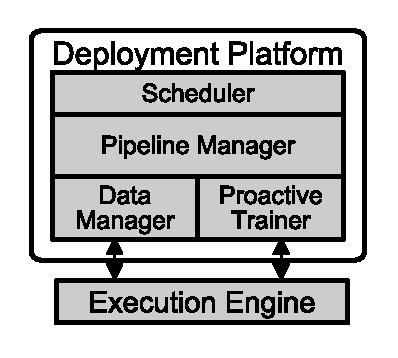
\includegraphics[width=\columnwidth]{../images/system-architecture.pdf}
\caption{System Architecture}
\label{fig:system-architecture}
\end{figure}

\subsection{Scheduler}\label{scheduler}
The scheduler component is responsible for scheduling a new proactive training.
The scheduler communicates with pipeline manager to instruct when to execute the proactive training.
The scheduler allows for two types of scheduling mechanism, namely \textit{static} and \textit{dynamic}.

The static scheduling uses a user-defined parameter that specifies the interval between executions of the proactive training.
This is a simple yet useful mechanism for use cases that require periodical updates of the model when the interval is known a priori (for example, every minute or hour). 
The dynamic scheduling tunes the scheduling interval based on the rate of the incoming prediction, prediction latency, and the time that it takes to execute the proactive training.
The scheduler uses the following formula to compute the time when to execute the proactive training:
\begin{center}
$T' = 2 * T * pr * pl$
\end{center}
where $T'$ indicates the time in seconds when the next iteration is scheduled to run, $T$ is the execution time of the last proactive training, $pl$ and $pr$ are the average prediction latency and the average number of prediction requests per second.
$T$ is measured by the scheduler component itself while $pr$ and $pl$ are measured by the deployment platform.
Using the formula to schedule the next proactive training, the scheduler ensures that all the prediction requests that arrived during the last proactive training and all new prediction requests are answered before a new iteration is scheduled.
Moreover, the scheduler assumes that the entire resources of the computing cluster are being used by the proactive trainer and therefore the prediction answering component is completely blocked while the proactive training is being executed.
By removing the above assumption, proactive training can be scheduled to execute more frequently.

\subsection{Data Manager} \label{data-manager}
The data manager component is responsible for storage of historical data, processing the incoming training data, and providing the proactive trainer with a new batch of training data for every iteration.

Historical data is typically large and may not fit in the memory or disk of a single machine. 
The data manager handles the communication with the underlying storage unit.
When new training data becomes available, the data manager appends the incoming data to the existing historical data.
Moreover, the incoming training data is forwarded to the pipeline manager to update the statistics required by the pipeline components.

When a new proactive training is scheduled to run, the data manager is responsible for providing the batch of training data.
A window size parameter specifies the amount of historical data that are to be sampled in the next proactive training.
Extreme values of the window size parameter are infinity, which means the data manager will sample the entire historical data and zero, which indicates that no historical data is used for proactive training.
After the sample is assembled, the recent training data is appended to the sample and the combination is provided to pipeline manager for next proactive training process.

Using zero or a small sampling window size uses more recent training data for training the model as compared to larger or infinity window size.
Different use cases may require different window size.
If older data are irrelevant to the training of the pipeline, setting window size to smaller values adapts the model to the newer data faster.
However, the incoming training data is not time-dependent, setting the sampling window size to larger or even infinity results in more stable models.
In our experiments, we investigate the effect of the different sampling window sizes on the quality of the model.

The data manager also allows for new training datasets to be registered while the model is being served.
The new dataset is merged with the existing historical data and immediately becomes available for next proactive training processes.

\subsection{Pipeline Manager} \label{pipeline-manager} 
The pipeline manager is the most important component of the system as it loads the pipeline trained offline, continuously trains the pipeline after deployment, evaluates the model update before applying the changes to the deployed model, and exposes the model to answer prediction queries.

Once a pipeline is deployed into the platform, the pipeline manager monitors the pipeline.
The scheduler component informs the pipeline to execute the next proactive training.
The pipeline manager then requests the data manager to provide the training dataset for the next proactive training.
Once the training dataset is received, the pipeline manager provides the proactive trainer component with the current model parameter and training dataset.
Once the training is over, the proactive trainer sends the updated model back to pipeline manager.
To ensure the quality of the model has not dropped, the pipeline manager uses an independent evaluation set to evaluate the quality of the model.
If the quality of the model does not degrade, the pipeline manager replaces the existing model with the new one.

When new training data arrives at the system, the data manager forwards the data to the pipeline manager. 
The pipeline manager directs the data through the pipeline one component at a time, where each component will receive the data, update their statistics, transform the data, and finally pass the transformed data to the next component.
The model training component of the pipeline is skipped as the model is updated separately in the proactive trainer component.
If the data materialization is enabled, the data processed by the pipeline is sent back to the data manager to be stored with the rest of the materialized data.
The data manager also forwards prediction requests to the pipeline manager.
Similar to training data, the pipeline manager also sends the prediction request through the pipeline to perform the necessary data processing.
Using the same pipeline to process both the training data and prediction requests guarantees that the same set of transformations are applied to both types of data (training and prediction requests) and prevents inconsistencies between training and serving that is a common problem in model deployment \cite{baylor2017tfx}.
After the prediction request is processed, the pipeline manager uses the model to make a prediction.

\subsection{Proactive Trainer} 
The proactive trainer is responsible for training the model by executing iterations of SGD.
It is also responsible for tuning the learning rate parameter of SGD.
In training process, the proactive trainer receives a training dataset and the initial model parameter from the pipeline manager, then performs one iteration of SGD and returns the updated model to the pipeline manager.
Although iterations are independent of each other, the proactive trainer needs to store the necessary information for computing the learning rate for next iterations.
The proactive trainer is the only component that is tightly coupled with the execution engine as it directly executes the code on the engine.
Therefore, separate implementations have to be provided for the different execution engines.

\subsection{Execution Engine}
All of the components of our deployment platform described so far, except for the proactive trainer, are decoupled from the execution engine.
In our deployment platform, any data processing platform capable of processing data both in batch mode (for continuous training) and streaming mode (answering prediction requests) is a suitable execution engine.
Apache Spark \cite{zaharia2010spark} is a distributed data processing platforms that can support both stream and batch data processing.
It works with data in memory and on disk which speeds up the execution of the proactive training.

\textit{Current Prototype.}
In our current prototype, we are using Apache Spark \cite{zaharia2010spark} as the execution engine.
The data manager component uses Hadoop Distributed File System (HDFS) for storing the historical data \cite{shvachko2010hadoop}.
We also leverage some of the components of the machine learning library in Spark to implement the proactive trainer.
To enable real-time prediction answering we use Spark streaming \cite{zaharia2013discretized}.
Spark streaming allows us to define the parallelism parameter ($pn$) and extract prediction requests rate and latency ($pr$ and $pl$).
The job scheduler uses these parameters to schedule new a new proactive training.
